As seen in the previous chapter, high accuracy applications are under continuous development. There are multiple options for free and public high accuracy corrections\cite{galileoHasPolicy}. Some examples from \cite{galileoHasPolicy} are:
\begin{itemize}
    \item Japanese QZSS is free over Japan. It provides centimeter-level accuracy
    \item European Galileo, Chinese Beidou and Russian GLONASS aim to provide similar accuracy for free in the upcoming years.
    \item Australia is developing the National Positioning Infrastructure Capability (NPIC) for 3-centimeters accuracy.
    \item International GNSS Service (IGS) provides high accuracy data for free.
    \item National and regional authorities which intend to provide high accuracy data for free.
\end{itemize}

Galileo High Accuracy Service (HAS) aims to provide PPP corrections for free, worldwide, via satellite links. According to \cite{galileoHasPolicy}, some characteristics of Galileo HAS are:
\begin{itemize}
    \item High Accuracy corrections transmitted for free, using an open standard format via the new Galileo E6-B signal with the possibility to transmit via terrestrial networks at the same time.
    \item The navigation messages will contain error corrections for satellite orbits, clocks, code and phase biases.
    \item The system will focus on Galileo and in the future it is possible to be extended to other GNSS.
    \item The service will be global with the possibility to include a regional augmentation over EU for ionospheric corrections.
    \item The positioning accuracy will be less than two decimeters.
\end{itemize}

The corrections will be included in the Galileo E6-B signal and will be transmitted by around $80\%$ of the satellites\cite{galileoHasPolicy}. The signal characteristics are presented in table \ref{table:1}
\begin{table}[h!]
\centering
\begin{tabular}{| m{15em} | m{20em} |}
    \hline
    \multicolumn{2}{|c|}{Signal and Data features} \\
    \hline
    Frequency & 1278.75 MHz \\
    \hline
    Signal & E6B \\
    \hline
    Min. Power & -158 dBW \\
    \hline
    Chip Rate & 5.115 Mcps \\
    \hline
    Code Length & 1 ms \\
    \hline
    Symbol Rate & 1000 sps \\
    \hline
    Data Rate & 492 bps \\ 
    \hline
    HA Data Rate & 448 bps \\
    \hline
    Data Coding & FEC as per Galileo OS ICD + interleaving $123 \times 8$ \\
    \hline
    Spreading Code Encryption & No \\
    \hline
    Data & Orbit and clock corrections, code and phase biases, flags, ionospheric information \\
    \hline
\end{tabular}
\caption{Galileo HAS E6B signal and data features. Source: \cite{galileoSisIcd}}
\label{table:1}
\end{table}

\subsection{Galileo E6 Signals}
\label{subsec:e6signals}

Paper \cite{e6breceiver} presents the E6B and E6C signals used in the Galileo HAS. The E6B and E6C signals are already being transmitted by satellites in orbit. The E6B signal will provide 492 bits per second per satellite of PPP corrections. This band allocation is new for GNSS and some reception and demodulation difficulties can be expected due to interference with radio amateurs, radars and due to the high bit-rate of the transmission\cite{e6breceiver}. However, This new band also comes with many new opportunities. The frequency is well separated from both E1 and E5 and the high bandwidth allows the transmission of corrections. The importance of frequency separation for ionosphere error elimination has been presented in \cite{instantPPP}.

The E6 Galileo signal is spread in two components \cite{e6breceiver}:
\begin{itemize}
    \item The data component (E6B), a modulo-two addition of FEC encoded data stream modulated by Binary Phase Shift. Keying (BPSK)
    \item The Pilot component (E6C), modulo-two addition of a code sequence with BPSK modulation.
\end{itemize}

\begin{table}[h!]
\centering
\begin{tabular}{| c | c | c |}
    \hline
    & E6B & E6C \\
    \hline
    Component & Data & Pilot \\
    \hline
    Carrier Frequency & 1278.75 Mhz & 1278.75 Mhz \\
    \hline
    Signal Polarization & RHCP & RHCP \\
    \hline
    Modulation & BPSK & BPSK \\
    \hline
    Chip Rate & 5.115 Mcps & 5.115 Mcps\\
    \hline
    Primary Code Length & 5115 chips & 5115 chips \\
    \hline
    Secondary Code Length & N/A & 100 chips \\
    \hline
    Secondary Code Length & N/A & 100 ms \\
    \hline
    Symbol Rate & 1000 sps & N/A \\
    \hline
    Data Rate & 492 bps & N/A\\
    \hline
    Data interleaving & $123 \times 8$ & N/A\\
    \hline
    Spreading Code Encryption Capability & Yes & Yes \\
    \hline
    Power Sharing & 50\% & 50 \% \\
    \hline
    Received minimum power & -155 dBW & -155 dBW \\
    \hline
\end{tabular}
\caption{Galileo E6 Properties. Source: \cite{e6breceiver}}
\label{table:2}
\end{table}

\begin{figure}[h]
\centering
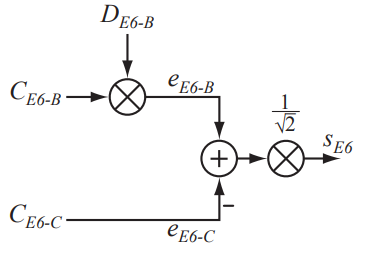
\includegraphics[scale=0.7]{img/signal_generation.png}
\caption{E6 Signal Generation, Source:\cite{e6breceiver}}
\label{fig:signal_generation}
\end{figure}

The E6 signal characteristics can be found in table \ref{table:2}. The signal generation diagram is presented in figure \ref{fig:signal_generation}. Before the data signal enters the mixer, a logic 0 bit is mapped to +1 signal level and a logic 1 bit is mapped to -1 signal level\cite{e6breceiver}.

\subsection{Galileo E6-B Data Structure}
\label{subsec:e6data}

As presented here, the data component of the E6 signal is transmitted via the E6B signal. In table \ref{table:2} we can see that the data is sent at 1000 symbols per second. Out of these 1000 symbols, the first 16 are the synchronization pattern. The remaining 984 symbols encode 492 data bits using Forward Error Correction (FEC). The data bits contain the PPP corrections. The corrections data will rely on external providers \cite{e6breceiver}. 


